% Chapter 7: K\"{o}nigsberg Bridges and Graph Theory
% ch07_konigsberg.tex

\chapter{The K\"{o}nigsberg Bridges and the Birth of Graph Theory}

\begin{historical}
In 1736, Euler solved the K\"{o}nigsberg bridges problem, proving that no walk exists crossing
each bridge exactly once. This paper, ``Solutio problematis ad geometriam situs pertinentis,''
is considered the founding document of graph theory and topology. Euler introduced the concept
of an Eulerian path and circuit, and established the fundamental criterion for their existence.
The problem was posed to Euler by the citizens of K\"{o}nigsberg (now Kaliningrad, Russia), who
wished to know if a certain walk was possible. Euler's solution revealed that the question
depended only on the connectivity of the land masses, not on their shapes or sizes. \cite{euler1736}\end{historical}

\section{The Problem}

The city of K\"{o}nigsberg had seven bridges connecting four land masses (two riverbanks and
two islands). The question: Is there a walk that crosses each bridge exactly once?

Euler abstracted this to a graph problem: Can we traverse every edge exactly once?

\begin{figure}[H]
\centering
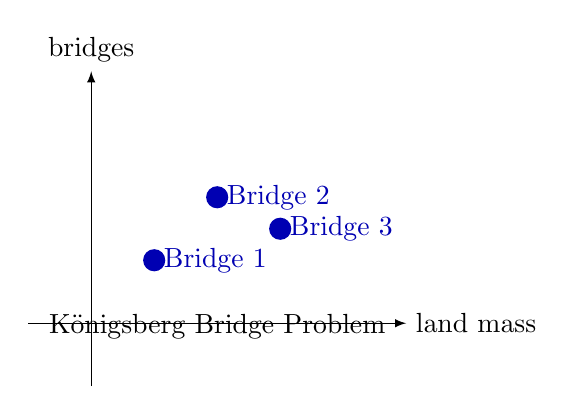
\begin{tikzpicture}[scale=0.8]
  \draw[->, >=latex] (-1,0) -- (5,0) node[right] {land mass};
  \draw[->, >=latex] (0,-1) -- (0,4) node[above] {bridges};
  \fill[blue!70!black] (1,1) circle (5pt) node[right] {Bridge 1};
  \fill[blue!70!black] (2,2) circle (5pt) node[right] {Bridge 2};
  \fill[blue!70!black] (3,1.5) circle (5pt) node[right] {Bridge 3};
  \node[below] at (2,0.3) {K\"{o}nigsberg Bridge Problem};
\end{tikzpicture}
\caption{Abstract graph representation of the K\"{o}nigsberg bridges}
\end{figure}

The K\"{o}nigsberg bridges connect four land masses labeled $A, B, C, D$. The bridge configuration is:
\begin{itemize}
\item Two bridges between $A$ and $B$
\item Two bridges between $A$ and $C$
\item One bridge between $A$ and $D$
\item One bridge between $B$ and $D$
\item One bridge between $C$ and $D$
\end{itemize}

This gives degrees: $\deg(A) = 5$, $\deg(B) = 3$, $\deg(C) = 3$, $\deg(D) = 3$.
Since all four vertices have odd degree, no Eulerian path exists.

\section{Euler's Theorem and Proofs}

\begin{theorem}[Euler's Bridge Theorem]
A connected graph has an Eulerian path (traversing every edge exactly once) if and only if
it has 0 or 2 vertices of odd degree.
\end{theorem}

\begin{proof}
Consider a walk that traverses every edge exactly once. Each time the walk enters a vertex
via one edge and leaves via another, it uses two edges incident to that vertex. Therefore,
every vertex visited (except possibly the start and end) must have even degree.
The start and end vertices can have odd degree (contributing one unused edge each).
Thus, the number of odd-degree vertices is either 0 (closed path) or 2 (open path).

Conversely, if a graph has 0 or 2 odd-degree vertices, an Eulerian path exists. The case
of 0 odd-degree vertices gives an Eulerian circuit (closed path), while 2 odd-degree vertices
gives an Eulerian path from one odd vertex to the other.
\end{proof}

\begin{theorem}[Degree Sum Formula]
For any undirected graph $G = (V, E)$:
\[
\sum_{v \in V} \deg(v) = 2|E|
\]
\end{theorem}

\begin{proof}
Each edge contributes exactly 2 to the sum of degrees (one for each endpoint). Therefore
the sum of all degrees equals twice the number of edges.
\end{proof}

\begin{corollary}
Any graph has an even number of odd-degree vertices.
\end{corollary}

\begin{proof}
From the degree sum formula, $2|E|$ is even. The sum of degrees is the sum of even-degree
vertices plus the sum of odd-degree vertices. For the total to be even, the number of
odd-degree vertices must be even.
\end{proof}

\begin{lstlisting}[caption={Checking Eulerian path existence}, label=lst:konigsberg]
from euler import eulerian_path_exists, eulerian_circuit_exists

# K\"{o}nigsberg configuration
bridges = [
    (1, 2), (1, 2), (1, 3), (1, 4),
    (2, 3), (2, 4), (3, 4)
]

adjacency = {vertex: [] for vertex in range(1, 5)}
for u, v in bridges:
    adjacency[u].append(v)
    adjacency[v].append(u)

print("K\"{o}nigsberg bridges analysis:")
print(f"  Has Eulerian path: {eulerian_path_exists(adjacency)}")
print(f"  Has Eulerian circuit: {eulerian_circuit_exists(adjacency)}")

# Analyze degrees directly from the adjacency list
degrees = {}
for u, v in bridges:
    degrees[u] = degrees.get(u, 0) + 1
    degrees[v] = degrees.get(v, 0) + 1
print(f"  Vertex degrees: {degrees}")
print(f"  Odd degree vertices: {sum(1 for d in degrees.values() if d % 2 == 1)}")
\end{lstlisting}

\section{Eulerian Circuits vs. Paths}

\begin{itemize}
\item \textbf{Eulerian circuit:} Closed path starting and ending at the same vertex
\item \textbf{Eulerian path:} Open path with distinct start and end vertices
\item \textbf{Condition:} Circuit exists iff all vertices have even degree
\end{itemize}

\begin{table}[H]
\centering
\begin{tabular}{l|c|c}
Property & Eulerian Circuit & Eulerian Path \\
\hline
All degrees even & Yes & Not required \\
Odd-degree vertices & 0 & 0 or 2 \\
Start vertex & Any even-degree & Odd-degree (if exists) \\
End vertex & Same as start & Other odd-degree \\
\end{tabular}
\caption{Comparison of Eulerian circuit and path conditions}
\label{tab:eulerian_comparison}
\end{table}

\section{Graph Representation}

Euler's insight was to abstract the geography into a graph:
\begin{itemize}
\item Vertices represent land masses
\item Edges represent bridges
\item Degree of a vertex = number of bridges connected to that land mass
\end{itemize}

For K\"{o}nigsberg: All four vertices have odd degree (5, 3, 3, 3), so no Eulerian path exists.

\section{Hierholzer's Algorithm}

Hierholzer's algorithm finds an Eulerian path in $O(E)$ time:

\begin{enumerate}
\item Start at a vertex with odd degree (or any vertex if all have even degree)
\item Follow edges, removing them as you go, until you return to the start
\item If any vertices remain unvisited, start a new cycle from a vertex on the current path
\item Combine cycles by splicing
\end{enumerate}

\begin{lstlisting}[caption={Hierholzer's algorithm}, label=lst:hierholzer]
from euler import hierholzer_algorithm

# Find Eulerian path in a graph that has one
graph = {
    'A': ['B', 'C'],
    'B': ['A', 'C', 'D'],
    'C': ['A', 'B', 'D'],
    'D': ['B', 'C']
}

path = hierholzer_algorithm(graph)
print(f"Eulerian path: {' -> '.join(path)}")
\end{lstlisting}

\section{Graph Eigenvalues and Spectral Analysis}

The eigenvalues of a graph's adjacency matrix provide deep insights into its structure.
For a graph $G$ with adjacency matrix $A$, the eigenvalues $\lambda_1 \geq \lambda_2 \geq \cdots \geq \lambda_n$
satisfy important properties:

\begin{theorem}[Spectral Properties]
For a $d$-regular graph with $n$ vertices:
\begin{itemize}
\item $\lambda_1 = d$ (the degree)
\item $|\lambda_i| \leq d$ for all $i$
\item The graph is connected iff $\lambda_1 > \lambda_2$
\end{itemize}
\end{theorem}

\begin{theorem}[Trace Formula]
For any graph:
\[
\text{tr}(A^k) = \sum_{i=1}^{n} \lambda_i^k = k \cdot (\text{number of closed walks of length } k)
\]
In particular, $\text{tr}(A^2) = 2|E|$ and $\text{tr}(A^3) = 6 \cdot (\text{number of triangles})$.
\end{theorem}

\begin{lstlisting}[caption={Eigenvalue analysis of graph}, label=lst:eigenvalues]
import numpy as np
from scipy.linalg import eigvals

# Adjacency matrix of a sample graph
A = np.array([
    [0, 1, 1, 0],
    [1, 0, 1, 1],
    [1, 1, 0, 1],
    [0, 1, 1, 0]
])

eigenvalues = eigvals(A)
print(f"Eigenvalues: {np.sort(eigenvalues)[::-1].real}")
print(f"Sum of eigenvalues: {np.sum(eigenvalues):.2f} (should be 0)")
print(f"Sum of squares: {np.sum(eigenvalues**2):.2f} (should be 2*E={2*5})")
\end{lstlisting}

\section{Applications of Euler's Theorem}

\begin{itemize}
\item \textbf{Network design:} Determining if a network can be traversed completely
\item \textbf{Route optimization:} Mail delivery, garbage collection routes
\item \textbf{DNA sequencing:} Overlap graphs for reconstructing DNA strands
\item \textbf{Urban planning:} Street sweeping, snow plowing routes
\item \textbf{PCB manufacturing:} Tracing paths on circuit boards without crossing
\end{itemize}

\section{Euler's Formula for Planar Graphs}

For connected planar graphs:
\[
V - E + F = 2
\]
where $V$ = vertices, $E$ = edges, $F$ = faces (including the outer face).

\begin{theorem}[Euler's Planar Graph Formula]
If $G$ is a connected planar graph with $V \geq 3$ vertices and $E$ edges, then:
\[
E \leq 3V - 6
\]
\end{theorem}

\begin{proof}
For a maximal planar graph (triangulation), each face has exactly 3 edges, and each edge
belongs to exactly 2 faces. Therefore $3F = 2E$. Substituting into Euler's formula:
$V - E + \frac{2E}{3} = 2$, which gives $E = 3V - 6$.
For any planar graph, $E \leq 3V - 6$.
\end{proof}

\begin{lstlisting}[caption={Euler's planar graph formula}, label=lst:euler_planar]
from euler import euler_formula_planar

# Tetrahedron (4 vertices, 6 edges, 4 faces)
print(f"Tetrahedron: V-E+F = {4-6+4} (should be 2)")

# Cube (8 vertices, 12 edges, 6 faces)
print(f"Cube: V-E+F = {8-12+6} (should be 2)")

# Dodecahedron (20 vertices, 30 edges, 12 faces)
print(f"Dodecahedron: V-E+F = {20-30+12} (should be 2)")
\end{lstlisting}

\section{Planar Graphs and Kuratowski's Theorem}

A graph is planar if and only if it contains no subgraph that is a subdivision of $K_5$
(complete graph on 5 vertices) or $K_{3,3}$ (complete bipartite graph). This is Kuratowski's
theorem (1930), building on Euler's work.

\begin{theorem}[Kuratowski's Theorem]
A finite graph is planar if and only if it does not contain a subgraph that is a subdivision
of $K_5$ or $K_{3,3}$.
\end{theorem}

\begin{figure}[H]
\centering
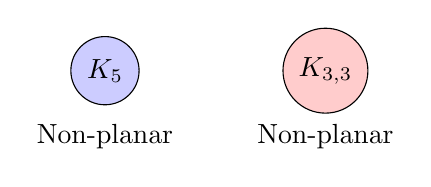
\begin{tikzpicture}[scale=0.7]
  \node[circle,draw,fill=blue!20] (a) at (0,0) {$K_5$};
  \node[circle,draw,fill=red!20] (b) at (4,0) {$K_{3,3}$};
  \node[below] at (0,-0.8) {Non-planar};
  \node[below] at (4,-0.8) {Non-planar};
\end{tikzpicture}
\caption{The two forbidden minors for planarity}
\end{figure}

\section{Computational Complexity}

\subsection{Checking Eulerian Properties}
\begin{itemize}
\item Computing degrees: $O(V + E)$
\item Checking odd-degree count: $O(V)$
\item Finding Eulerian path (Hierholzer's algorithm): $O(E)$
\end{itemize}

\subsection{Planar Graph Formula}
\begin{itemize}
\item Verifying $V - E + F = 2$: $O(1)$ after counting
\item Finding $F$: Requires traversal (DFS/BFS), $O(V + E)$
\end{itemize}

\section{Generalizations}

\subsection{Directed Graphs}
For directed graphs, an Eulerian circuit exists if and only if:
\begin{itemize}
\item The graph is strongly connected
\item In-degree equals out-degree for every vertex
\end{itemize}

\subsection{Mixed Graphs}
For graphs with both directed and undirected edges, the problem is NP-complete in general.

\section{The Chinese Postman Problem}

The Chinese Postman Problem asks: given a connected graph, find the shortest closed walk
that traverses every edge at least once.

\subsection{Chinese Postman Algorithm}
\begin{enumerate}
\item If the graph is Eulerian, return the Eulerian circuit
\item Find all odd-degree vertices
\item Find minimum-weight perfect matching among odd-degree vertices
\item Add duplicated edges corresponding to the matching
\item Find Eulerian circuit in the augmented graph
\end{enumerate}

\section{Frequently Asked Questions}

\begin{itemize}
\item \textbf{Q: Why does the K\"{o}nigsberg problem have no solution?} \\
All four land masses have odd degree (3 bridges each). Euler's theorem states that an Eulerian path requires 0 or 2 odd-degree vertices. Since K\"{o}nigsberg has 4, no such path exists.

\item \textbf{Q: What's the difference between an Eulerian path and a Hamiltonian path?} \\
An Eulerian path traverses every \emph{edge} exactly once. A Hamiltonian path visits every \emph{vertex} exactly once. The latter is much harder to determine---it's NP-complete.

\item \textbf{Q: How does Euler's theorem apply to real-world routing?} \\
Street sweepers, garbage trucks, and snow plows need to traverse every street. If the street graph has 0 or 2 odd-degree vertices, an optimal route exists. Otherwise, some streets must be traversed twice (the Chinese Postman Problem).

\item \textbf{Q: Can we add bridges to make K\"{o}nigsberg solvable?} \\
Adding one bridge between any two odd-degree vertices reduces both to even degree, giving exactly 2 odd vertices and an Eulerian path. Adding two bridges between all four would give all even degrees and an Eulerian circuit.

\item \textbf{Q: What is the relationship to the Four Color Theorem?} \\
Euler's formula for planar graphs ($V - E + F = 2$) was a key step in proving the Four Color Theorem. The theorem states that any planar map can be colored with 4 colors so that no adjacent regions share the same color.

\item \textbf{Q: What is the Chinese Postman Problem?} \\
Given a graph, find the shortest closed walk that traverses every edge at least once. This is a generalization of the Eulerian circuit problem where some edges may need to be traversed twice.

\item \textbf{Q: How does this relate to network design?} \\
In network design, determining whether a network can be traversed (for inspection, maintenance, etc.) requires checking for Eulerian properties. This has applications in circuit board testing, database traversal, and robot path planning.

\item \textbf{Q: What is the spectral gap of a graph?} \\
The spectral gap $\lambda_1 - \lambda_2$ measures how well-connected a graph is. A large spectral gap indicates good expansion properties and fast mixing times for random walks.
\end{itemize}

\section{Exercises}

\begin{exercise}
Prove that a connected graph with exactly 2 odd-degree vertices has an Eulerian path.
\end{exercise}

\begin{exercise}
Show that the Petersen graph has no Eulerian path.
\end{exercise}

\begin{exercise}
For a connected planar graph with $V$ vertices and $E$ edges, prove $E \leq 3V - 6$.
\end{exercise}

\begin{exercise}[Computational]
Implement Hierholzer's algorithm to find an Eulerian path in a graph that has one.
\end{exercise}

\begin{exercise}
Determine the minimum number of additional bridges needed to make the K\"{o}nigsberg graph Eulerian.
\end{exercise}

\begin{exercise}
Prove that a graph has an Eulerian circuit if and only if every vertex has even degree and the graph is connected.
\end{exercise}

\begin{exercise}
Show that a directed graph has an Eulerian circuit if and only if it is strongly connected and in-degree equals out-degree at every vertex.
\end{exercise}

\begin{exercise}
Prove that every planar graph has a vertex of degree at most 5.
\end{exercise}

\begin{exercise}[Computational]
Implement the Chinese Postman Algorithm to find the shortest route that traverses every edge of a given graph at least once.
\end{exercise}

\begin{exercise}
Show that the number of edges in a planar graph with $V \geq 3$ satisfies $E \leq 3V - 6$.
\end{exercise}

\begin{exercise}
Prove that a $d$-regular graph with adjacency matrix $A$ has $\lambda_1 = d$ as its largest eigenvalue.
\end{exercise}

\begin{exercise}[Computational]
Compute the eigenvalues of the adjacency matrix for the complete graph $K_n$ and verify that $\lambda_1 = n-1$ and $\lambda_2 = \cdots = \lambda_n = -1$.
\end{exercise}

\begin{exercise}
Show that the number of triangles in a graph equals $\frac{1}{6}\text{tr}(A^3)$, where $A$ is the adjacency matrix.
\end{exercise}

\begin{exercise}
Prove that for any graph, the sum of eigenvalues equals zero.
\end{exercise}

\begin{exercise}[Computational]
Verify Euler's formula $V - E + F = 2$ for several planar graphs by constructing their embeddings and counting faces.
\end{exercise}
